\documentclass[12pt,fleqn]{article}\usepackage{../../common}
\begin{document}
Materyel Mekaniği - 11


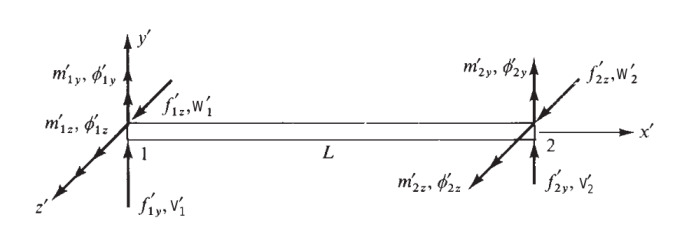
\includegraphics[width=25em]{phy_020_strs_11_01.jpg}

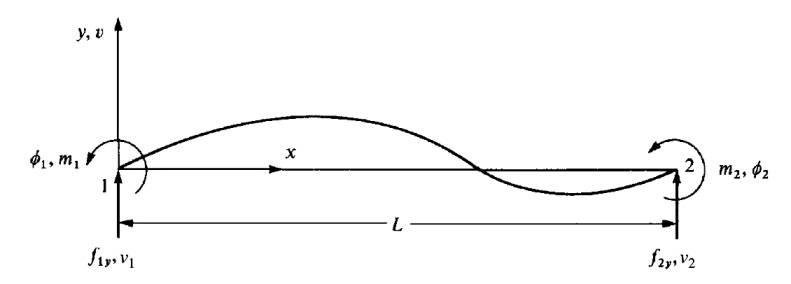
\includegraphics[width=25em]{phy_020_strs_11_02.jpg}

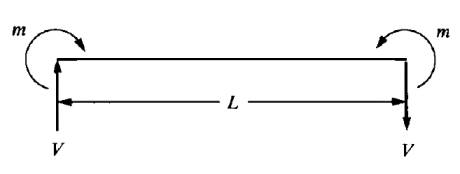
\includegraphics[width=25em]{phy_020_strs_11_03.jpg}


$x-z$ düzlemi

$$
\frac{EI_y}{L^4}
\left[\begin{array}{cccc}
12L & -6L  & -12L & -6L^2 \\
    & 4L^3 & 6L^2 & 2L^3  \\
    &      & 12L  & 6L^2  \\
    &      &      & 4L^3
\end{array}\right]
$$

$x-y$ düzlemi

$$
\frac{EI_y}{L^4}
\left[\begin{array}{cccc}
12L & 6L  & -12L & 6L^2 \\
    & 4L^3 & -6L^2 & 2L^3  \\
    &      & 12L  & -6L^2  \\
    &      &      & 4L^3
\end{array}\right]
$$




\begin{minted}[fontsize=\footnotesize]{python}
from sympy import symbols, pprint, latex
from sympy.matrices import Matrix
import pandas as pd
pd.set_option('display.max_columns', None)

all_vars = ['u1','v1','w1','phi1x','phi1y','phi1z',\
            'u2','v2','w2','phi2x','phi2y','phi2z']
A,G,J,E,L,Iy,Iz = symbols("A,G,J,E,L,Iy,Iz")
\end{minted}

\begin{minted}[fontsize=\footnotesize]{python}
# x-z
vars1 = ['w1','phi1y','w2','phi2y']
M1 = pd.DataFrame([[12*L, -6*L**2,-12*L,-6*L**2],
                  [-6*L**2,4*L**3,6*L**2,2*L**3],
                  [-12*L,6*L**2,12*L,6*L**2],
                  [-6*L**2,2*L**3,6*L**2,4*L**3]],index=vars1)
M1.columns = vars1
M1 = M1 * (E*Iy/L**4 )
# x-y
vars2 = ['v1','phi1z','v2','phi2z']
M2 = pd.DataFrame([[12*L, 6*L**2,-12*L,6*L**2],
                  [6*L**2,4*L**3,-6*L**2,2*L**3],
                  [-12*L,-6*L**2,12*L,-6*L**2],
                  [6*L**2,2*L**3,-6*L**2,4*L**3]],index=vars2)
M2.columns = vars2
M2 = M2 * (E*Iz/L**4 )

# Eksenel Yuk
vars3 = ['u1','u2']
M3 = pd.DataFrame([[1,-1],[-1,1]],index=vars3)
M3.columns = vars3
M3 = M3 * (A*E/L)

# Burulma (Torsion)
vars4 = ['phi1x','phi2x']
M4 = pd.DataFrame([[1,-1],[-1,1]],index=vars3)
M4.columns = vars4
M4 = M4 * (G*J/L)
\end{minted}

\begin{minted}[fontsize=\footnotesize]{python}
import sys; sys.path.append('../phy_020_strs_08')
import dfutil

M1f = dfutil.expand_dataframe(M1,all_vars)
M2f = dfutil.expand_dataframe(M2,all_vars)
M3f = dfutil.expand_dataframe(M3,all_vars)
M4f = dfutil.expand_dataframe(M4,all_vars)
Mall = M1f + M2f + M3f + M4f
\end{minted}

Sonuç matrisini bir dosyaya yazalım, 

\begin{minted}[fontsize=\footnotesize]{python}
Mall = Mall.apply(np.vectorize(lambda x: latex(x)))
fout = open('matrix1.tex','w')
fout.write ('$$\\left[\\begin{array}{cccccccccccc}')
fout.write('\n')
for x,y in Mall.iterrows():
   row = ' & '.join(list(y)) + '\\\\'
   row = row.replace('0.0','0')
   fout.write(row)
   fout.write('\n')
fout.write ('\\end{array}\\right]$$')
fout.close()
\end{minted}

Ve altta belgeye dahil edelim,

$$
\left[\begin{array}{cccccccccccc}
\mathtt{\text{\textbackslashfrac\{A E\}\{L\}}} & \mathtt{\text{0}} & \mathtt{\text{0}} & \mathtt{\text{0}} & \mathtt{\text{0}} & \mathtt{\text{0}} & \mathtt{\text{- \textbackslashfrac\{A E\}\{L\}}} & \mathtt{\text{0}} & \mathtt{\text{0}} & \mathtt{\text{0}} & \mathtt{\text{0}} & \mathtt{\text{0}}\\
\mathtt{\text{0}} & \mathtt{\text{\textbackslashfrac\{12 E Iz\}\{L\textasciicircum\{3\}\}}} & \mathtt{\text{0}} & \mathtt{\text{0}} & \mathtt{\text{0}} & \mathtt{\text{\textbackslashfrac\{6 E Iz\}\{L\textasciicircum\{2\}\}}} & \mathtt{\text{0}} & \mathtt{\text{- \textbackslashfrac\{12 E Iz\}\{L\textasciicircum\{3\}\}}} & \mathtt{\text{0}} & \mathtt{\text{0}} & \mathtt{\text{0}} & \mathtt{\text{\textbackslashfrac\{6 E Iz\}\{L\textasciicircum\{2\}\}}}\\
\mathtt{\text{0}} & \mathtt{\text{0}} & \mathtt{\text{\textbackslashfrac\{12 E Iy\}\{L\textasciicircum\{3\}\}}} & \mathtt{\text{0}} & \mathtt{\text{- \textbackslashfrac\{6 E Iy\}\{L\textasciicircum\{2\}\}}} & \mathtt{\text{0}} & \mathtt{\text{0}} & \mathtt{\text{0}} & \mathtt{\text{- \textbackslashfrac\{12 E Iy\}\{L\textasciicircum\{3\}\}}} & \mathtt{\text{0}} & \mathtt{\text{- \textbackslashfrac\{6 E Iy\}\{L\textasciicircum\{2\}\}}} & \mathtt{\text{0}}\\
\mathtt{\text{0}} & \mathtt{\text{0}} & \mathtt{\text{0}} & \mathtt{\text{\textbackslashfrac\{G J\}\{L\}}} & \mathtt{\text{0}} & \mathtt{\text{0}} & \mathtt{\text{0}} & \mathtt{\text{0}} & \mathtt{\text{0}} & \mathtt{\text{- \textbackslashfrac\{G J\}\{L\}}} & \mathtt{\text{0}} & \mathtt{\text{0}}\\
\mathtt{\text{0}} & \mathtt{\text{0}} & \mathtt{\text{- \textbackslashfrac\{6 E Iy\}\{L\textasciicircum\{2\}\}}} & \mathtt{\text{0}} & \mathtt{\text{\textbackslashfrac\{4 E Iy\}\{L\}}} & \mathtt{\text{0}} & \mathtt{\text{0}} & \mathtt{\text{0}} & \mathtt{\text{\textbackslashfrac\{6 E Iy\}\{L\textasciicircum\{2\}\}}} & \mathtt{\text{0}} & \mathtt{\text{\textbackslashfrac\{2 E Iy\}\{L\}}} & \mathtt{\text{0}}\\
\mathtt{\text{0}} & \mathtt{\text{\textbackslashfrac\{6 E Iz\}\{L\textasciicircum\{2\}\}}} & \mathtt{\text{0}} & \mathtt{\text{0}} & \mathtt{\text{0}} & \mathtt{\text{\textbackslashfrac\{4 E Iz\}\{L\}}} & \mathtt{\text{0}} & \mathtt{\text{- \textbackslashfrac\{6 E Iz\}\{L\textasciicircum\{2\}\}}} & \mathtt{\text{0}} & \mathtt{\text{0}} & \mathtt{\text{0}} & \mathtt{\text{\textbackslashfrac\{2 E Iz\}\{L\}}}\\
\mathtt{\text{- \textbackslashfrac\{A E\}\{L\}}} & \mathtt{\text{0}} & \mathtt{\text{0}} & \mathtt{\text{0}} & \mathtt{\text{0}} & \mathtt{\text{0}} & \mathtt{\text{\textbackslashfrac\{A E\}\{L\}}} & \mathtt{\text{0}} & \mathtt{\text{0}} & \mathtt{\text{0}} & \mathtt{\text{0}} & \mathtt{\text{0}}\\
\mathtt{\text{0}} & \mathtt{\text{- \textbackslashfrac\{12 E Iz\}\{L\textasciicircum\{3\}\}}} & \mathtt{\text{0}} & \mathtt{\text{0}} & \mathtt{\text{0}} & \mathtt{\text{- \textbackslashfrac\{6 E Iz\}\{L\textasciicircum\{2\}\}}} & \mathtt{\text{0}} & \mathtt{\text{\textbackslashfrac\{12 E Iz\}\{L\textasciicircum\{3\}\}}} & \mathtt{\text{0}} & \mathtt{\text{0}} & \mathtt{\text{0}} & \mathtt{\text{- \textbackslashfrac\{6 E Iz\}\{L\textasciicircum\{2\}\}}}\\
\mathtt{\text{0}} & \mathtt{\text{0}} & \mathtt{\text{- \textbackslashfrac\{12 E Iy\}\{L\textasciicircum\{3\}\}}} & \mathtt{\text{0}} & \mathtt{\text{\textbackslashfrac\{6 E Iy\}\{L\textasciicircum\{2\}\}}} & \mathtt{\text{0}} & \mathtt{\text{0}} & \mathtt{\text{0}} & \mathtt{\text{\textbackslashfrac\{12 E Iy\}\{L\textasciicircum\{3\}\}}} & \mathtt{\text{0}} & \mathtt{\text{\textbackslashfrac\{6 E Iy\}\{L\textasciicircum\{2\}\}}} & \mathtt{\text{0}}\\
\mathtt{\text{0}} & \mathtt{\text{0}} & \mathtt{\text{0}} & \mathtt{\text{- \textbackslashfrac\{G J\}\{L\}}} & \mathtt{\text{0}} & \mathtt{\text{0}} & \mathtt{\text{0}} & \mathtt{\text{0}} & \mathtt{\text{0}} & \mathtt{\text{\textbackslashfrac\{G J\}\{L\}}} & \mathtt{\text{0}} & \mathtt{\text{0}}\\
\mathtt{\text{0}} & \mathtt{\text{0}} & \mathtt{\text{- \textbackslashfrac\{6 E Iy\}\{L\textasciicircum\{2\}\}}} & \mathtt{\text{0}} & \mathtt{\text{\textbackslashfrac\{2 E Iy\}\{L\}}} & \mathtt{\text{0}} & \mathtt{\text{0}} & \mathtt{\text{0}} & \mathtt{\text{\textbackslashfrac\{6 E Iy\}\{L\textasciicircum\{2\}\}}} & \mathtt{\text{0}} & \mathtt{\text{\textbackslashfrac\{4 E Iy\}\{L\}}} & \mathtt{\text{0}}\\
\mathtt{\text{0}} & \mathtt{\text{\textbackslashfrac\{6 E Iz\}\{L\textasciicircum\{2\}\}}} & \mathtt{\text{0}} & \mathtt{\text{0}} & \mathtt{\text{0}} & \mathtt{\text{\textbackslashfrac\{2 E Iz\}\{L\}}} & \mathtt{\text{0}} & \mathtt{\text{- \textbackslashfrac\{6 E Iz\}\{L\textasciicircum\{2\}\}}} & \mathtt{\text{0}} & \mathtt{\text{0}} & \mathtt{\text{0}} & \mathtt{\text{\textbackslashfrac\{4 E Iz\}\{L\}}}\\
\end{array}\right]
$$

Kaynaklar

[1] Bayramlı, {\em Fizik, Materyel Mekanigi 7}

[2] Logan, {\em A First Course in the Finite Element Method, 6th Ed}


\end{document}



